\documentclass[10.9pt,a4paper]{article}
\usepackage[utf8]{inputenc}
\usepackage[spanish]{babel}
\usepackage[T1]{fontenc}
\usepackage[left=1in, right=1in, top=1in, bottom=1in]{geometry}
%\usepackage{fancyhdr}
%\pagestyle{fancy}
\usepackage{graphicx}
\usepackage[colorlinks=false]{hyperref}
\usepackage{color}
%\usepackage{indentfirst}
%\usepackage{wrapfig}
%\usepackage{lipsum}
\pagenumbering{gobble} % omite la numeracion de las páginas
\usepackage{fontawesome}
\usepackage{pdfpages}
%\renewcommand{\rmdefault}{phv} % Arial
%\renewcommand{\sfdefault}{phv} % Arial
%\rhead{}
%\lhead{}
%\chead{Igreja Presbiteriana Central\\ Rua Albert Scharlet, 376 - Coronel Fabriciano/MG \\ CEP: 35170-038 Tel: 31.99728-4312}
%\lfoot{www.egmon.com.br}
%\cfoot{\thepage}
%\rfoot{}
\title{ISLP}
%\author{}
\usepackage{fancyhdr} %activamos el paquete
\pagestyle{fancy} %seleccionamos un estilo
 \lfoot{\begin{footnotesize}
\hfill\\
2970 Avenida Arce, Zona San Jorge \\
La Paz - Bolivia\\
 \end{footnotesize}}

\rfoot{\begin{footnotesize}
\hrule 
\faEnvelopeO \url{fundacion@aru.org.bo} \\
\url{https://www.aru.org.bo/} \\
\faPhone: 22004492 22004491 \\ 
 \end{footnotesize}} 
 
 \rhead{
\includegraphics[scale=0.5]{islp} } %texto izquierda de la cabecera
 \lhead{
\includegraphics[scale=0.25]{arulogo} } %texto izquierda de la cabecera
%\thispagestyle{empty}

\begin{document}
\hfill
\vspace{0.7cm}\\

\hspace{5.5cm} \today \\

Señor: Carlos Henríquez PhD 

\textbf{CENTRO LATINOAMERICANO DE ESTADÍSTICA APLICADA}
\vspace{0.1cm}\\


\begin{tabular}{lp{10cm}}
\hspace{5cm} & \textbf{Asunto}: Invitación de patrocinio para la \textbf{Competencia Boliviana de Posters Estadísticos 2018-2019.}\\
\end{tabular}

\hfill

De nuestra mayor consideración.\\

Durante los meses de Mayo de 2018 a Enero de 2019 se llevará a cabo la \textbf{Primera Competencia Boliviana de Posters Estadísticos}, esta competencia es parte del `Proyecto Internacional de Alfabetización Estadística'' (ISLP), ésta fue lanzada a inicios de 2018 y está abierta a estudiantes de escuelas y universidades de todo el mundo. Los ganadores de las competencias nacionales pasan a concursar en la competencia internacional. La competencia en Bolivia es coordinada por Fundación Aru y el ISLP, actualmente se realizan tareas de preparación.\\

Reconocemos el compromiso de su institución con la promoción de la estadística en el País, por ello \textbf{Invitamos a que su institución forme parte de los patrocinadores de esta competencia}. El patrocinio puede estar vinculado a una o más de las siguientes características:

\begin{itemize}
\item \textbf{Material de apoyo:} Se refiere a publicaciones, material de escritorio personalizados u otros. 
\item \textbf{Difusión:} Involucra el poder tener espacios publicitarios de la competencia en los medios que dispongan los patrocinadores; Pagina web, radio, redes sociales, etc. También incluye la posibilidad de emplear el logo de su institución en los medios de difusión de la competencia.
\item \textbf{Bases de datos:} Los patrocinadores pueden poner a disposición del los concursantes sus bases de datos, para ser empleadas en los Posters.
\item \textbf{Fondos para la competencia:} El objetivo es tener un fondo de aportes de los patrocinadores que permita dar soporte a los gastos de organización y premiación. Al finalizar la competencia se realizará una rendición de cuenta y los saldos serán destinados a la próxima competencia.
\end{itemize}

El soporte de los patrocinadores permitirá hacer sostenible la competencia a largo plazo y brindará una oportunidad a los patrocinadores de visibilizarce como instituciones que apoyan los procesos de Alfabetización Estadística en Bolivia. \\

Le solicitamos pueda confirmar la participación de su institución hasta el 31 de Julio del presente. Si desea tener una reunión para conocer más acerca del proyecto o intercambiar ideas no dude en contactarnos a \faEnvelopeO: \url{achirino@aru.org.bo} -  \faPhone: 70694453 o visitarnos a la página de la ''Competencia de Posters Bolivianos'' \faGoogle:  \url{https://islp-bolivia.github.io/}.\\

Atentamente:

%\marginpar{Coloca anotações na margem}

\begin{center}
\vspace{0.1cm}


\includegraphics[scale=0.8]{firmaPaul}\hspace{5.7cm}


\noindent \hspace{0.2cm}Paul Villarroel Via \hspace{2.7cm}				Alvaro Chirino Gutierrez\\
\hspace{0.5cm}Director Fundación Aru \hspace{1.7cm}	Coordinador Nacional ISLP

\end{center}

\newpage

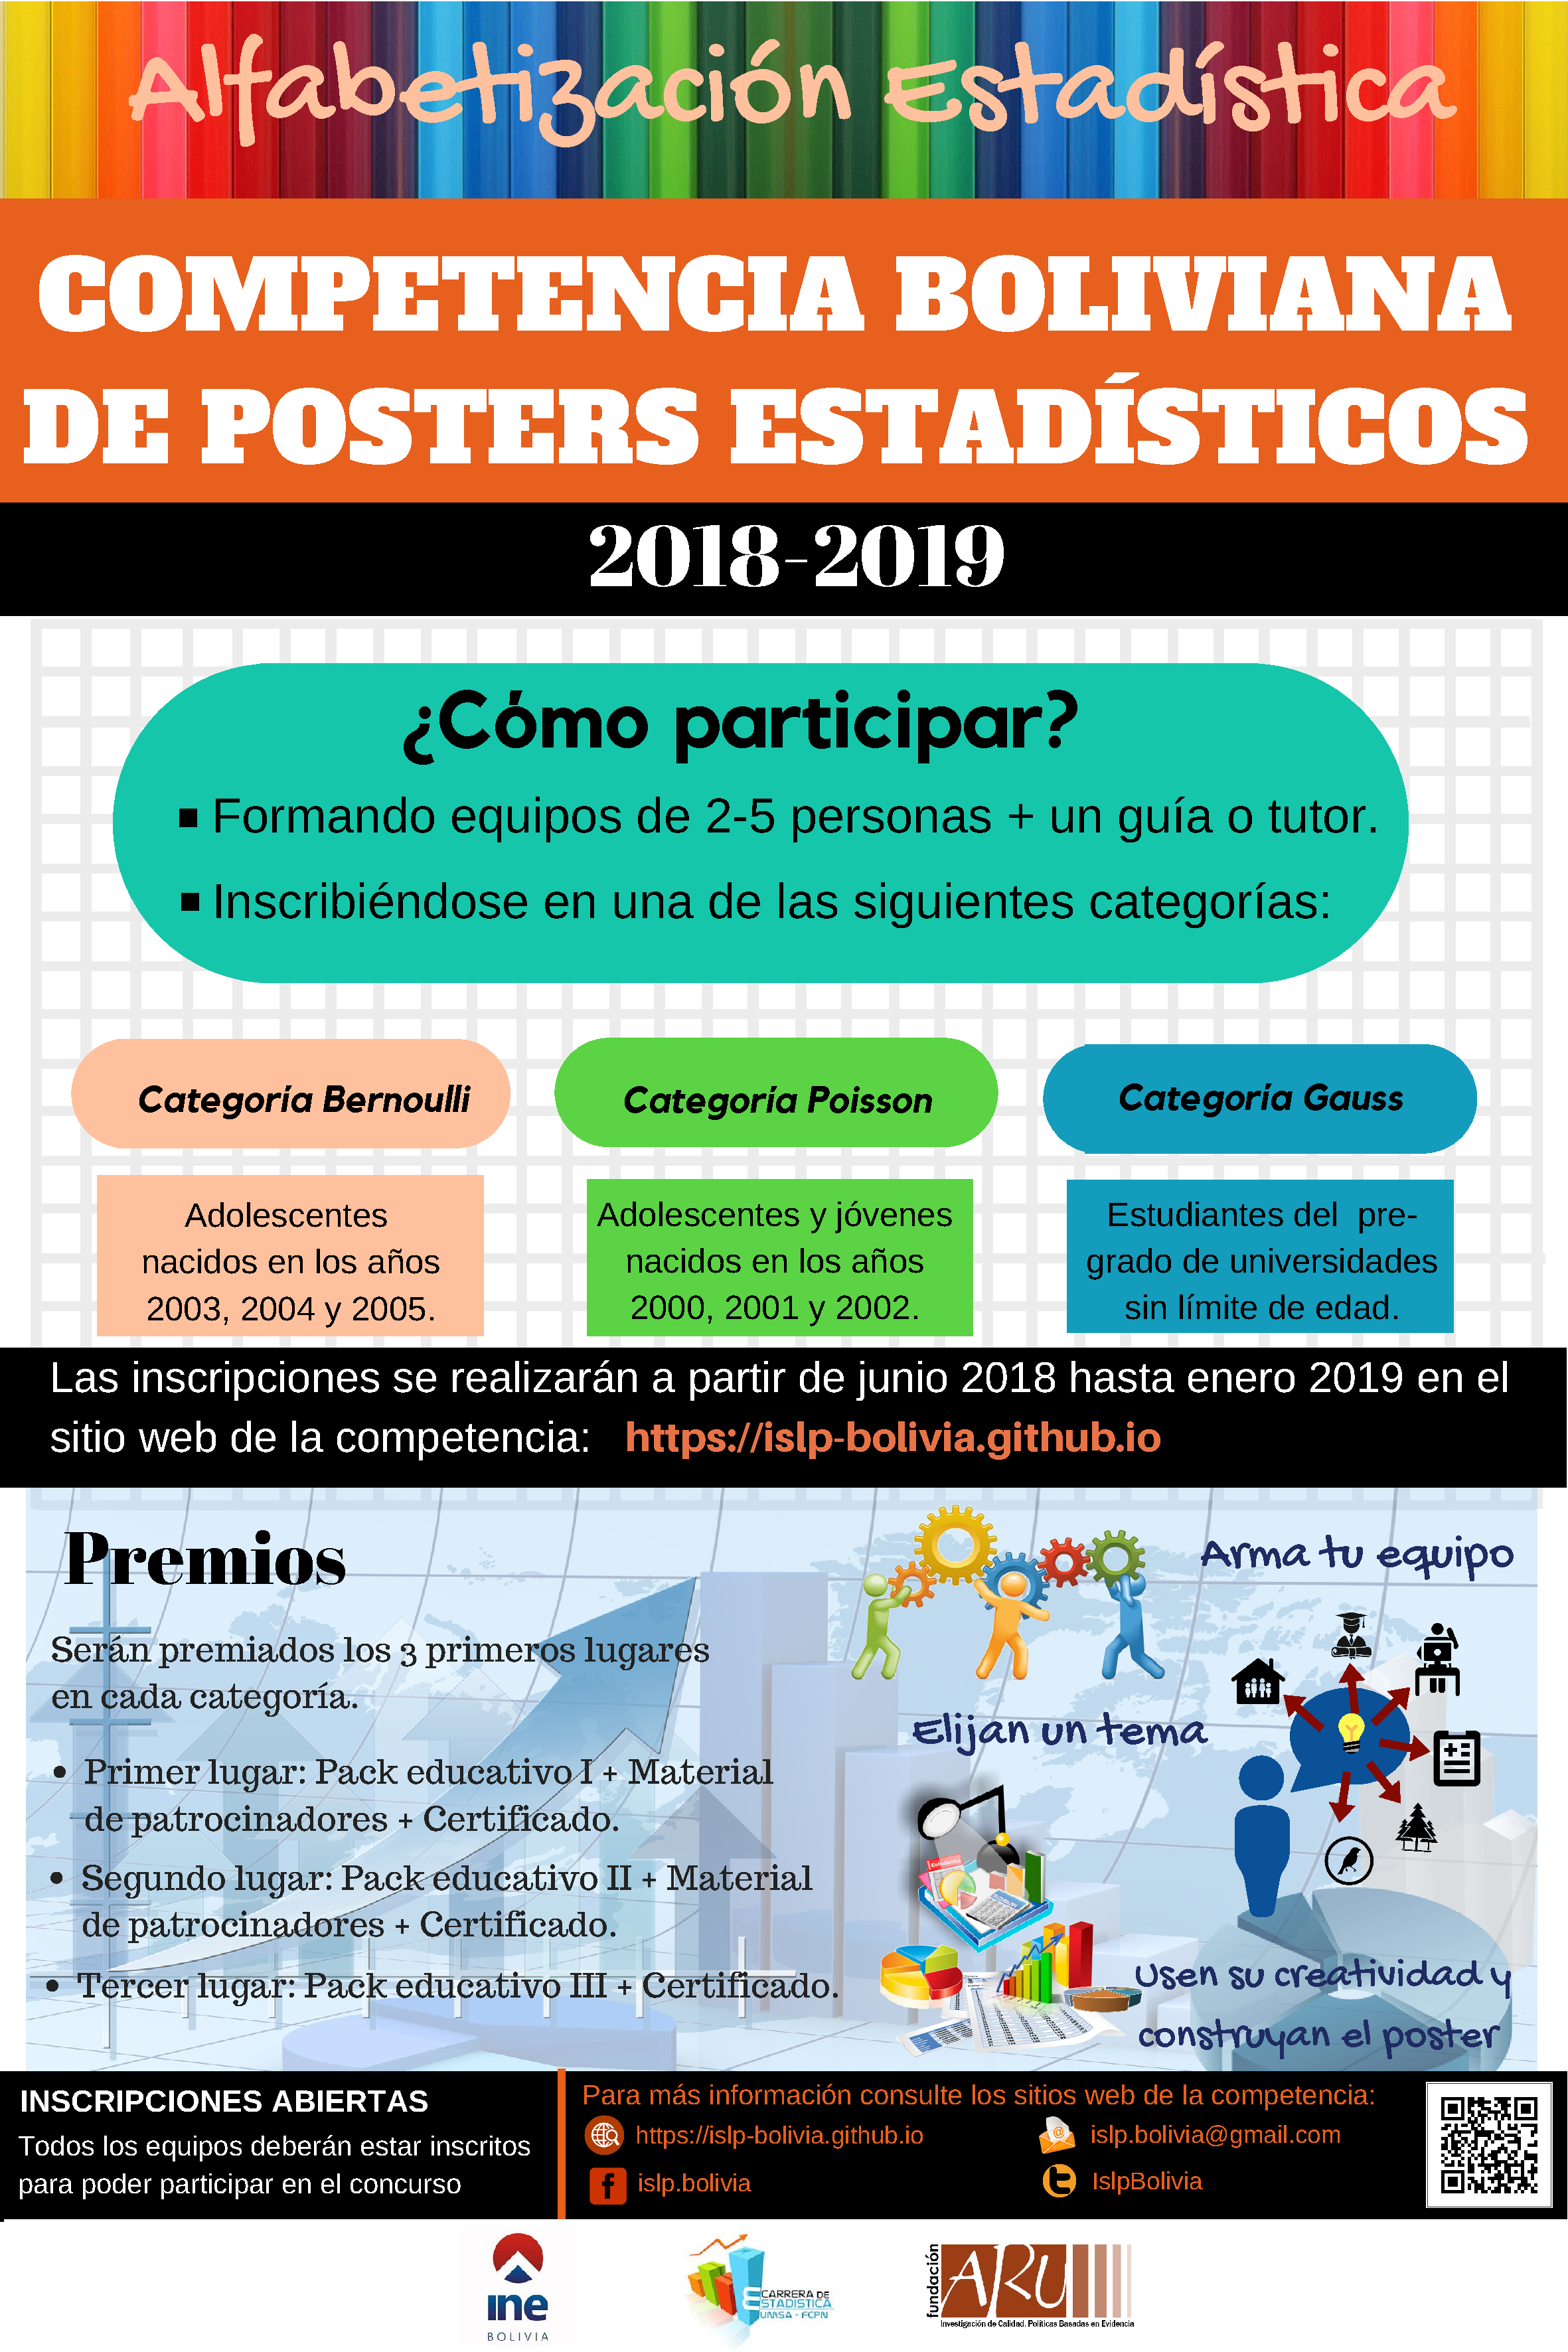
\includepdf[pages=-]{poster.pdf}
\end{document}